\section{Auswertung}

\subsection{Emissionsspektrum der Kupfer-Röntgenröhre}

Das Emissionsspektrum der Kupfer-Röntgenröhre wurde mit einer Integrationszeit von $\increment t = \SI{10}{\second}$ in jeweils $\increment \theta = 0{,}1\textdegree$ Abständen gemessen.
Diese Zählraten am Geiger-Müllerzählrohr lassen sich nun im Diagramm \ref{fig:plot1} in Abhängigkeit vom Winkel $\theta$ darstellen.
Der Bremsberg ist im Diagramm durch schwarze Punkte dargestellt, sie zeigen die Strahlung welche durch Abbremsung der Elektronen am Kupfer entsteht. 
Außerdem sind zwei charakteristische Linien zu erkennen, die $K_{\beta}$ und $K_{\alpha}$-Linie.

\begin{figure}[h]
  \centering
  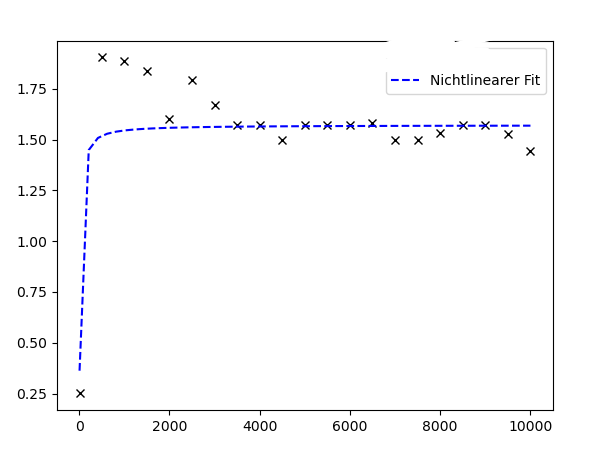
\includegraphics[width=\textwidth]{build/plot1.pdf}
  \caption{Röntgenspektrum einer Kupfer-Röntgenröhre.}
  \label{fig:plot1}
\end{figure}

Diese Linien lassen sich am Diagramm \ref{fig:plot1} und den gemessenen Werten in Tabelle \ref{tab:cuwerte1} grob ablesen zu.

\begin{align*}
K_{\alpha} &= 22{,}5\textdegree \\
K_{\beta} &= 20{,}2\textdegree
\end{align*}
Aus diesen Winkeln lässt sich mit der aufgestellten Beziehung \eqref{eqn:braggEnergy} die Energie dieser K-Linien berechnen. Hierbei wird die Beugungsordnung $n = 1$ betrachtet.
Es ergeben sich die Werte.
\begin{align}
\label{eqn:q1}
E_{\text{K,}\alpha} &= \SI{8.043}{\kilo\electronvolt} \\
\label{eqn:q2}
E_{\text{K,}\beta} &= \SI{8.914}{\kilo\electronvolt}
\end{align}
Die Abweichungen zu den angegebenen Literaturwerten \ref{tab:vorbereitung} sind in der folgenden Tabelle \ref{tab:litabweichung1} in Prozent angegeben.
\begin{table}
\centering
\caption{Prozentuale Abweichung zu den Literaturwerten.}
\label{tab:litabweichung1}
\begin{tabular}{c c c}
    \toprule
    Linie & Energieabweichung & Winkelabweichung \\
    \midrule
    $K_{\alpha}$     &  $\SI{0.058}{\percent}$ &  $\SI{0.044}{\percent}$    \\
     $K_{\beta}$     &  $\SI{0.081}{\percent}$ &  $\SI{0.099}{\percent}$   \\
    \bottomrule
\end{tabular}
\end{table}

\subsection{Bestimmung der Transmission}
In der Versuchsdurchführung wurden die Zählraten der Röntgenstrahlung mit einem Aluminium-Absorber $N_{Al}$ und ohne Absorber $N_{\text{ohne}}$ in $\increment \theta= 0.1\textdegree$ Abständen gemessen.
Diese Zählraten sind poissonverteilt und somit lässt sich der Fehler bezüglich jeder einzelnen Zählrate mit
\begin{equation*}
\increment N_{i} = \sqrt{N_{i}}
\end{equation*}
angeben. Die originalen Messwerte sowie die poissonverteilten Fehler sind in Tabelle \ref{tab:alu} angegeben. Diese Wertepaare können nun durch die angegebene Totzeitkorrektur in Gleichung \eqref{eqn:totzeit}
angepasst werden. Dazu werden die Werte mit der festen Totzeit $\tau = \SI{90}{\micro\second}$, wobei eine Gaußsche Fehlerfortpflanzung nötig wird. Diese ergibt sich wie folgt.
\begin{equation*}
\increment I = \left( \frac{1}{1 - \tau \cdot N} + \frac{\tau \cdot N_{i}}{(1 - \tau \cdot N_{i})^{2}} \right) \increment N_{i}
\end{equation*}
Die korrigierten Intensitätswerte sind nun zusammen mit ihrem Fehler in der Tabelle \ref{tab:korrektur} angegeben.
Für die erste Beugungsordnung gilt nach Gleichung \ref{eqn:lambda} ein direkter Zusammenhang zwischen dem Kristallwinkel und den Wellenlängen der Strahlung.
Mit dem Zusammenhang \eqref{eqn:wichtig} kann die Transmission bestimmt werden. Hierbei gilt.
\begin{equation*}
T = \frac{I_{Al}}{I_{\text{ohne}}}
\end{equation*}
Da beide Zählraten fehlerbehaftet sind kann zunächst wieder eine Fehlerfortpflanzung bestimmt werden, diese lautet.
\begin{equation*}
\increment T = \sqrt{\left( \frac{1}{I_{\text{ohne}}}\right)^{2} (\increment I_{Al})^{2} + \left( \frac{I_{Al}}{(I_{\text{ohne}})^{2}}\right)^{2} (\increment I_{\text{ohne}})^{2}}
\end{equation*}
Aus den Wellenlängen $\lambda$ und der Transmission $T$ lässt sich nun ein $\lambda$-$T$ Diagramm erstellen, die Wertepaare sind in Tabelle \ref{tab:VIVONZULUL} angegeben.

\begin{figure}[h]
  \centering
  \includegraphics[width=\textwidth]{build/plot2.pdf}
  \caption{Transmissionsdiagramm in Abhängigkeit von der Wellenlänge.}
  \label{fig:plot2}
\end{figure}

Bei der Bestimmung der Compton-Wellenlänge müssen einigen Transmissionswerten Wellenlängen zugeordnet werden, somit bietet es sich an eine lineare Ausgleichsgerade der
Form
\begin{equation*}
y = a \cdot x + b
\end{equation*}
durch die Werte zu legen.
Ein linearer Fit in Python liefert die folgenden Parameter.
\begin{align*}
a &= \SI{-0.152(2)}{{10^{11}}\per\meter}\\
b &= \SI{1.225(14)}{}\\
\end{align*}
Die Ausgleichsgerade
\begin{equation}
\label{eqn:gerade}
T = -0.152 \cdot \lambda + 1.225
\end{equation}
ist in das Diagramm \ref{fig:plot2} mit eingezeichnet und dadurch lassen sich die Wellenlängen leicht zuordnen. Wichtig ist hierbei,
dass $\lambda$ in der Größenordnung $10^{-11}$ herauskommt.

\subsection{Bestimmung der Compton-Wellenlänge}
Die Bestimmung der Compton-Wellenlänge basiert auf der Verschiebung der Wellenlänge und kann in diesem Versuch durch die Transmissionsverhältnisse
der ungestreuten und gestreuten Röntgenstrahlung ermittelt werden. Nach der Gleichung \eqref{eqn:wichtig} lässt sich die ungestreute Transmission schreiben als.
\begin{equation}
\label{eqn:d1}
T_{1} = \frac{I_{1}}{I_{\text{ohne}}}
\end{equation}
Analog gilt für die gestreute Transmission.
\begin{equation}
\label{eqn:d2}
T_{2} = \frac{I_{2}}{I_{\text{ohne}}}
\end{equation}
$I_{1}$ ist dabei die Intensität ohne Streuung, $I_{2}$ die Intensität mit Streuung  und $I_{0}$ die die Intensität ohne Absorber.
Die Werte aus der Tabelle \ref{tab:idky} wurden dabei in der Versuchsdurchführung gemessen.
Aus den Gleichungen \eqref{eqn:d1} und \eqref{eqn:d2} folgen die Transmissionswerte $T_{1}$ und $T_{2}$.
\begin{align*}
T_{1} &= 0.432 \\
T_{2} &= 0.375
\end{align*}
Eingesetzt in die Geradengleichung \eqref{eqn:gerade} liefern sie die zugehörigen Wellenlängen $\lambda$.
\begin{align}
\lambda_{1} &=  \SI{5.217e-11}{\meter} \\
\lambda_{2} &=  \SI{5.592e-11}{\meter} \\
\intertext{Der Wellenlängenunterschied nach Gleichung \eqref{eqn:diff} liefert nun die gesuchte Compton-Wellenlänge $\lambda_{c}$.}
\lambda_{c} &= \SI{3.758e-12}{\meter} 
\end{align}
Die prozentuale Abweichung vom Literaturwert aus Gleichung \eqref{eqn:comptontheoriewert} entspricht $\SI{54.89}{\percent}$.
\\
Eine Totzeitkorrektur ist bei kleinen Zählraten meist nicht vonnöten da der Nenner der Gleichung \eqref{eqn:totzeit} gegen 1 konvergiert und somit keine
Korrektur stattfindet. Dies liegt außerdem an der bereits sehr kleinen Totzeit von $\SI{90}{\micro\second}$ welche dazu führt, dass dieser schneller gegen 1 verläuft.
